\paragraph{Draft status.} Experiments are in progress. Counts below describe the registered protocol, not completed evaluations. Final tables will distinguish completed results, numerical qualification, and any failures.

\paragraph{Geometry and observations.}
The controlled object is a $240\times80\times80$\,mm deformable block with known canonical geometry, density $625$\,kg/m$^3$, and Poisson ratio $0.35$. Two position-controlled tools couple to unknown smooth Gaussian attachment footprints. The observed prefix contains three settled configurations: nominal tool poses, a 6\,mm right-tool translation along $y$, and a 6\,mm translation along $z$. A $640\times480$ rendered RGB-D marker pipeline provides the same 27 visible point positions to all methods. Known synthetic marker IDs establish correspondence; depth has independent 0.3\,mm Gaussian noise and image sampling introduces pixel quantization. The positional objective uses a common 0.3\,mm coordinate scale. No force, reaction, material, or attachment labels are supplied. Predictions are evaluated at 81 canonical query points, with visible and hidden-surface subsets reported separately.

\paragraph{Cohorts and shifts.}
The protocol declares nine development objects, twelve calibration objects, and three disjoint test cohorts: eighteen objects from the development parameter ranges, twelve with extrapolated elastic coefficients and spatial heterogeneity, and twelve with shifted environmental-field amplitude, center, width, and gravity direction. Material coefficients within development range from 8 to 40\,kPa, and total attachment stiffnesses from 1500 to 15000\,N/m. Each object has a new 3\,mm familiar-direction query, five new positional interaction patterns, and a doubled-amplitude query. New patterns include stretching, opposed tool motion, twisting, bending, and diagonal translation. An additional transfer challenge translates both tools together through the fixed spatial field. These are declared interaction and parameter shifts; the reference material law remains Neo-Hookean.

\paragraph{Numerical references.}
Reference geometry uses quadratic finite elements and independent spatial and quadrature refinement. Every action must have a displacement RMS change below 20\,$\mu$m, equilibrium residual below $10^{-9}$\,N, positive deformation Jacobians above $0.1$, and reaction balance below $10^{-7}$\,N. Maximum-coordinate refinement changes are retained separately, since localized attachment-edge behavior converges more slowly. Acceptance in an RMS norm does not certify pointwise stress convergence. The inverse predictor uses a smaller discretization and an independently checked dense tangent implementation. A development-only sharp-attachment pilot motivated the finite smooth footprint: its localized compression reached the Jacobian guard under refinement, whereas the smooth version retained substantial nonrigid deformation and passed the original numerical thresholds.

\paragraph{Comparisons.}
The physical baselines use official PhysTwin spring-mass and PhysGaussian material-point simulation components with documented adapters for the shared positional interface. They retain their own constitutive representations. PhysTwin learns per-spring parameters; the MPM adapter fits material variation, compliant tool coupling, and gravity direction. We tune initialization, discretization, and settling on development cases. A positional neural predictor is trained on a separate synthetic object bank, with an ID-action training variant and a separately reported variant exposed to all local action families. Controlled ablations fix environmental loading to its nominal value or freeze the spatial force at each material point's canonical position. The main predictor and neural comparisons cover all 42 declared test objects. The more expensive physical comparisons use the first six objects in each test cohort, giving two objects per attachment layout and an 18-object matched subset selected before test inference. Full Gaussian appearance reconstruction is outside this component benchmark.

\paragraph{Metrics and adaptation.}
The primary error is coordinate RMS displacement error,
\begin{equation}
 e=\sqrt{\frac{1}{3N}\sum_{i=1}^N\|\hat u_i-u_i\|_2^2}.
\end{equation}
We also report Euclidean point RMSE, hidden-surface error, and residual motion after removing the best rigid transform. Incremental error compares $\hat u(a)-\hat u(a_0)$ against $u(a)-u(a_0)$, separating the predicted response to the new action from static shape-completion error. Aggregation treats the object as the independent unit. Paired comparisons resample objects rather than frames or points. Probing compares a fixed $+40$\,mm $y$ translation, a reproducible random action, and the sensitivity-based policy, all with one additional acquired response and a separate $-40$\,mm $y$ target. Twelve independent calibration objects set separate pre- and post-acquisition interval scales; nine test objects evaluate transfer. A material-indexed-load ablation receives exactly the probe response selected for the spatial model.

\begin{figure*}[t]
\centering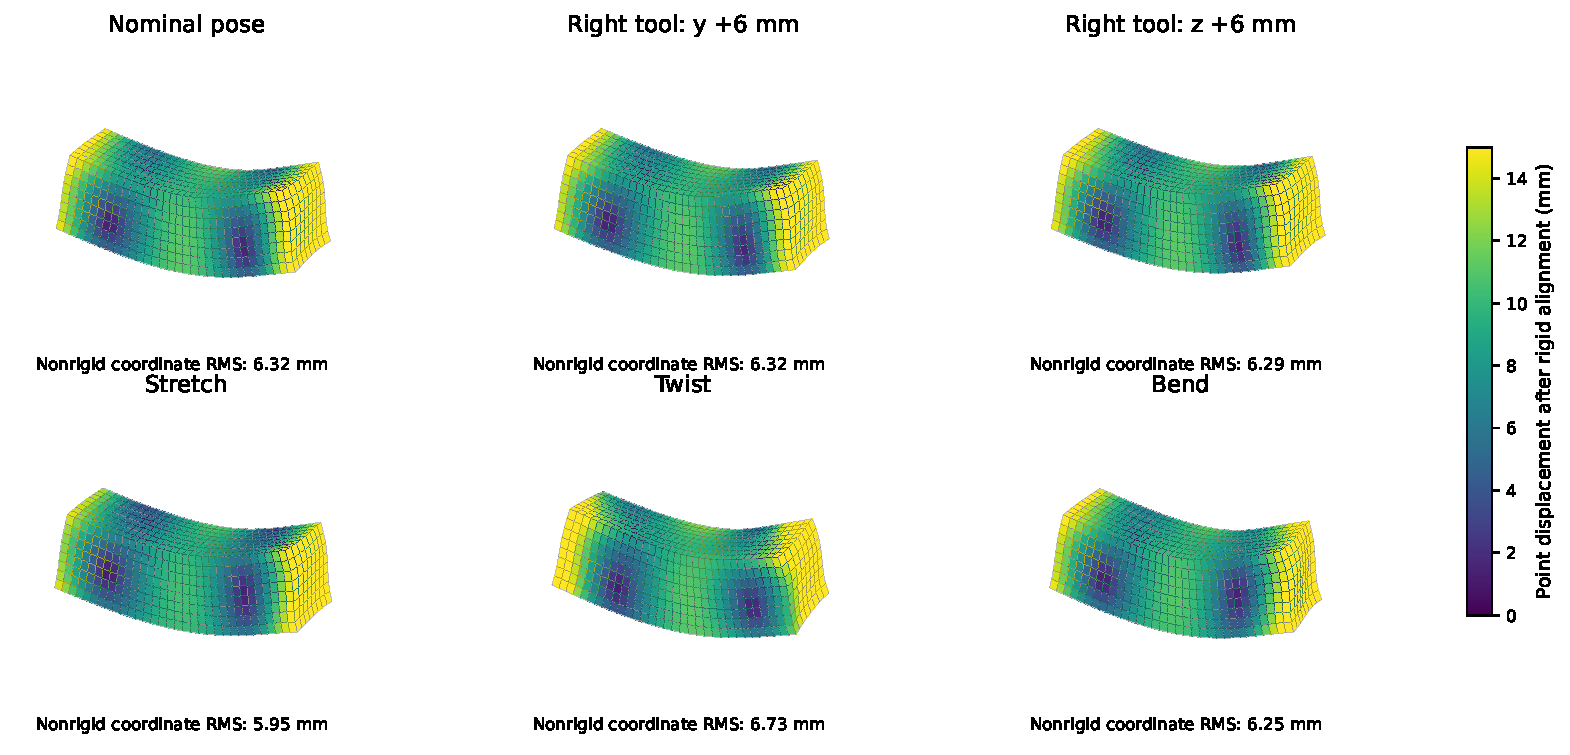
\includegraphics[width=\textwidth]{figures/scenarios.pdf}
\caption{Development reference geometry at actual deformation scale. The top row supplies the three observed configurations; the bottom row illustrates new positional interactions. Color measures displacement remaining after rigid alignment. The block has millimetre-scale nonrigid deformation, with no visual amplification.}
\label{fig:scenarios}
\end{figure*}
